\subsection*{Problema 33}
\textbf{Enunciado:} Calcular la integral:
\begin{equation*}
\int \dfrac{4x^4 - 2x^3 - x^2 + 3x + 1}{x^3 + x^2 - x - 1} \, dx
\end{equation*}

\textbf{Solución:} 
Primero, observemos que el grado del numerador es $4$ y el del denominador es $3$. Dado que el grado del numerador es mayor, realizamos la división polinómica. Dividiendo el numerador entre el denominador, obtenemos un cociente y un residuo:

\begin{align*}
\dfrac{4x^4 - 2x^3 - x^2 + 3x + 1}{x^3 + x^2 - x - 1} = \\
4x - 6 + \dfrac{9x^2 + 7x - 5}{x^3 + x^2 - x - 1}
\end{align*}

Ahora factorizamos el denominador agrupando términos:
\begin{align*}
x^3 + x^2 - x - 1 &= x^2(x + 1) - (x + 1) \\
&= (x^2 - 1)(x + 1) \\
&= (x + 1)^2(x - 1)
\end{align*}

Aplicamos fracciones parciales a la expresión restante:
\begin{align*}
\dfrac{9x^2 + 7x - 5}{(x + 1)^2(x - 1)} = \dfrac{A}{x + 1} + \dfrac{B}{(x + 1)^2} + \dfrac{C}{x - 1}
\end{align*}

Multiplicando por el denominador común:
\begin{align*}
9x^2 + 7x - 5 = &A(x + 1)(x - 1) \\
&+ B(x - 1) + C(x + 1)^2
\end{align*}

Evaluando en valores convenientes de $x$:
\begin{itemize}
    \item Si $x = 1$: $11 = 4C \implies C = \dfrac{11}{4}$
    \item Si $x = -1$: $-3 = -2B \implies B = \dfrac{3}{2}$
    \item Si $x = 0$: $-5 = -A - B + C$ \\
    $\implies A = 5 - \dfrac{3}{2} + \dfrac{11}{4} = \dfrac{25}{4}$
\end{itemize}

Sustituyendo los valores hallados, reescribimos la integral completa:
\begin{align*}
\int &\left( 4x - 6 + \dfrac{25/4}{x + 1} + \dfrac{3/2}{(x + 1)^2} + \dfrac{11/4}{x - 1} \right) dx
\end{align*}

Integramos término a término:
\begin{align*}
&= 2x^2 - 6x + \dfrac{25}{4}\ln|x + 1| \\
&\quad - \dfrac{3}{2(x + 1)} + \dfrac{11}{4}\ln|x - 1| + C
\end{align*}

\begin{figure}[H]
	\centering
	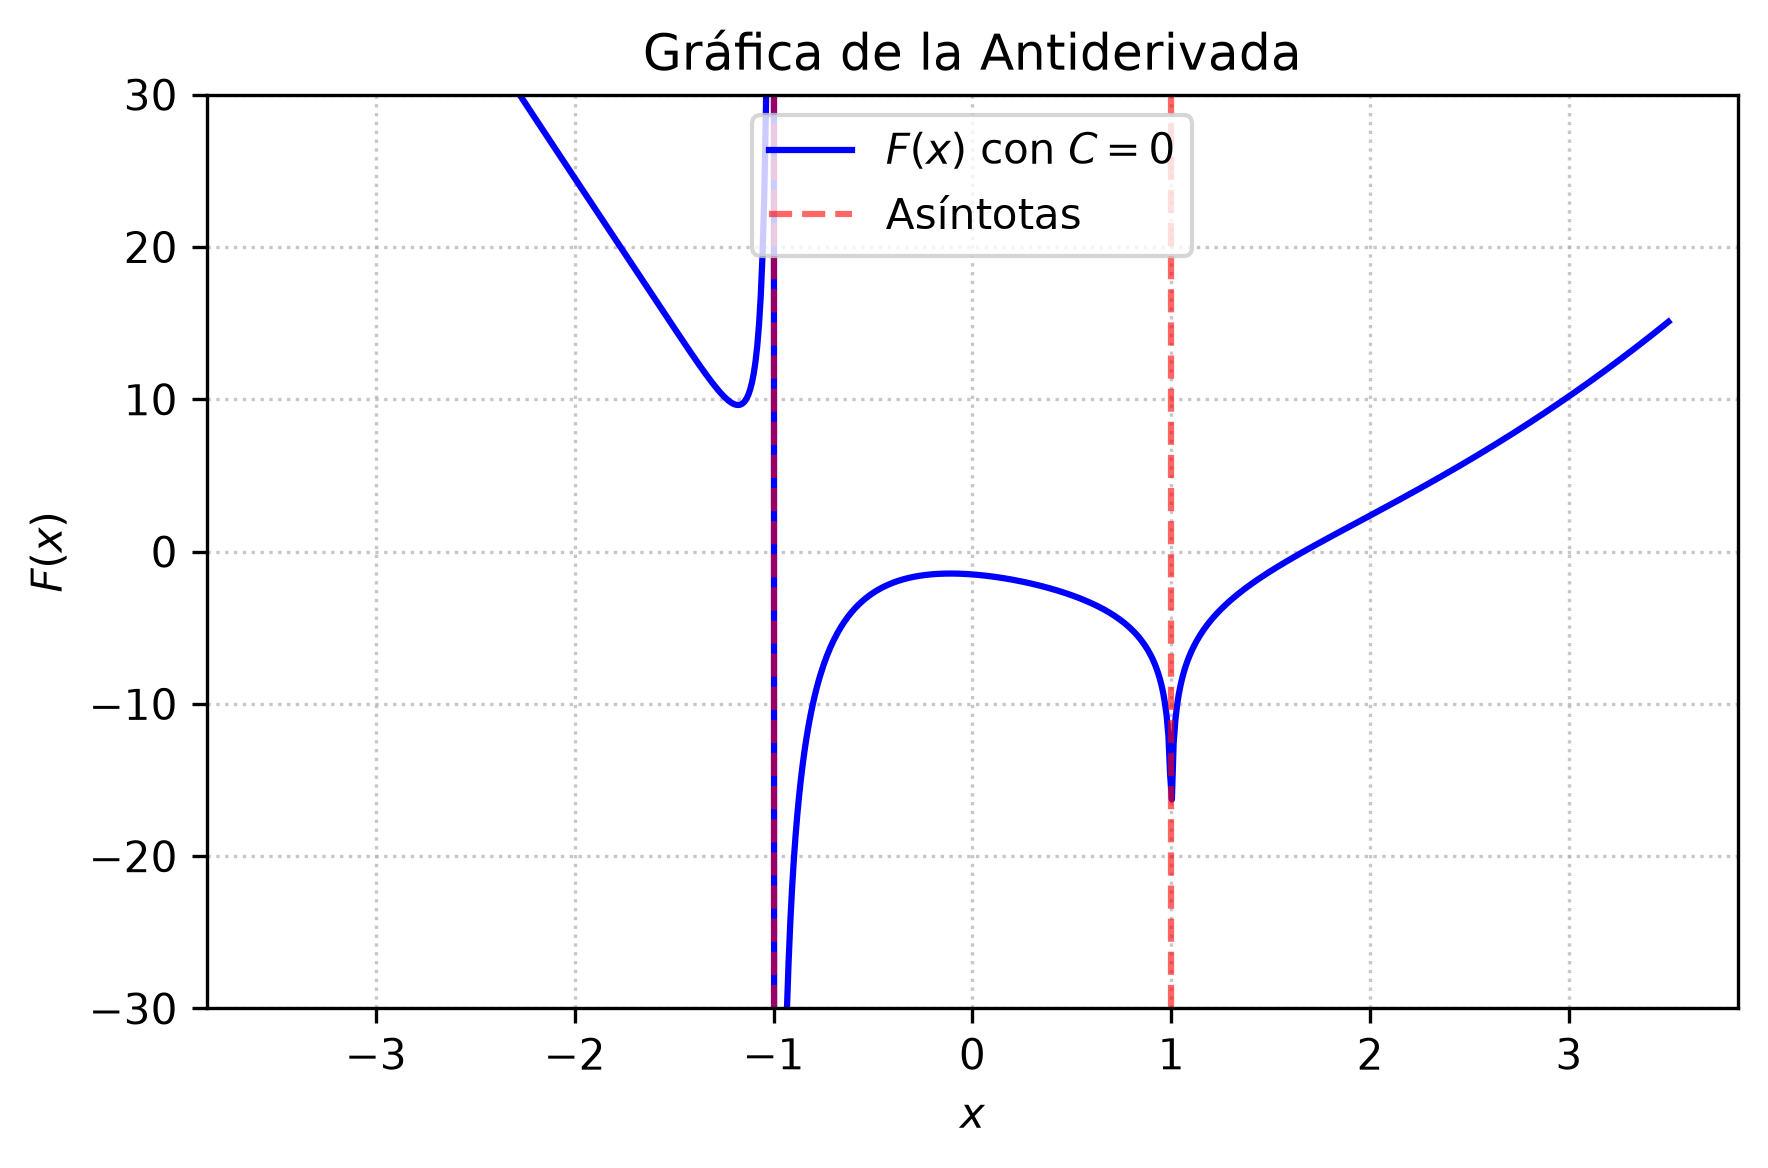
\includegraphics[width=\columnwidth]{semana_03/graficas/SEM03_P33_grafica.png}
	\caption{Representación gráfica de $f(x)$ y su antiderivada $F(x)$ evaluada para la constante de integración $C = 0$ (Problema 33).}
	\label{fig:problema33}
\end{figure}
